\documentclass[spanish]{assignment}

\usepackage{float}

% Title page
\title{Búsqueda y Minería de Información}
\subtitle{Práctica 4 - Sistemas de Recomendación y Análisis de Redes Sociales}
\author{Enrique Cabrerizo Fernández\\ Guillermo Ruiz Álvarez}
\date{\today}
\university{Universidad Autónoma de Madrid}

\begin{document}
	\makepre
	\section{Sistemas de recomendación}
	En esta sección se describirá la estructura y el diseño de los sistemas de recomendación implementados en esta práctica.
	Se han desarrollado dos sistemas de recomendación:
	\begin{itemize}
		\item Basados en contenido, utilizando Rocchio como método de recomendación.
		\item Basados en filtrado colaborativo por usuario, utilizando KNN como método de recomendación. 
	\end{itemize}
	En ambos sistemas se utiliza un \texttt{Min-Heap} para ordenar los resultados.
	
	\subsection{Estructura de datos utilizada}
	Para almacenar y operar los datos se han utilizado dos librerías externas.
	\begin{itemize}
		\item Se ha utilizado la clase \texttt{HashBasedTable} de \texttt{Guava} para el almacenamiento
		de datos en tablas. Estas tablas son equivalentes a una tabla hash con dos claves en lugar de una.
		\item Se ha utilizado la clase \texttt{SparseDoubleMatrix2D} de \texttt{Colt} para operar con los datos utilizando matrices dispersas. 
		
		Dado que estas matrices tienen un tamaño limitado, se han creado clases que a parte de almacenar los datos en la matriz tienen estructuras de datos (arrays y tablas hash) para poder obtener un identificador a partir de una fila (o columna) y una fila (o columna) a partir de un identificador.
	\end{itemize}
	
	\subsection{Modelo de ponderación de las etiquetas}
	El modelo que se ha utilizado para la ponderación de las etiquetas es el siguiente:
	\begin{itemize}
		\item Se han tomado los identificadores de las películas como identificadores de documentos.
		\item Se han tomado los identificadores de las etiquetas como identificadores de términos.
		\item Se han tomado los pesos de las etiquetas como la frecuencia de los términos en los respectivos documentos.
	\end{itemize}
	Una vez hecho esto, se ha creado una tabla donde el elemento $(i,j)$ es el $tf-idf(t_j, m_i)$, donde $t_j, m_i$ representa un término y una película, respectivamente.
	
	\newpage
	\subsection{Recomendación basada en contenido.}
	Para implementar el sistema de recomendación basada en contenido se ha creado una clase \texttt{ContentBased} que utiliza:
	\begin{itemize}
		\item La clase \texttt{MovieRatingData} para cargar la matriz de ratings, en la que las filas representan usuarios, las columnas películas, y los valores los correspondientes ratings.
		\item La clase \texttt{MovieContentData} para cargar la matriz de contenido, en la que las filas representan películas, las columnas etiquetas, y los valores el $tf-idf$ de cada película y etiqueta. 
		\item La clase \texttt{RocchioSimilarity} utilizada para generar y almacenar los valores de ranking de las peliculas aún no valoradas por un usuario.
	\end{itemize}
	
	\subsubsection{Sistema de recomendación - Rocchio}
	Dada una fila de la matriz de ratings, se calcula el centroide de un usuario realizando el siguiente producto:
	$$centroide(u) = c^u = \frac{1}{|u|}\vec{u}C$$
	donde $|u|$ es el número de películas valoradas por el usuario, $\vec{u}$ es la fila de la matriz de ratings correspondiente al usuario $u$ y $C$ es la matriz de contenido donde las películas están representadas por filas.
	
	Una vez obtenido el centroide, se realiza el coseno del mismo con todas las filas de la matriz de contenido que no hayan sido valoradas por el usuario, aplicando la fórmula:
	$$cos(c^u, m_i) = \frac{c^u\cdot m_i}{\sqrt{c^u\cdot c^u\times m_i\cdot m_i}}$$
	
	donde $m_i$ representa el vector fila de la matriz de contenido correspondiente a la película con índice $i$.
	
	\subsection{Recomendación basada en filtrado colaborativo.}
	Para implementar el sistema de recomendación basada en contenido se ha creado una clase \texttt{CollaborativeUserBased} que utiliza:
	\begin{itemize}
		\item La clase \texttt{MovieRatingData} para cargar la matriz de ratings, en la que las filas representan usuarios, las columnas películas, y los valores los correspondientes ratings.
		\item La clase \texttt{KNNSimilarity} utilizada para generar y almacenar los valores de rating de las peliculas aún no valoradas por un usuario.
	\end{itemize}
	
	\subsubsection{Sistema de recomendación - KNN}
	Se han realizado dos implementaciones del cálculo de similitudes para este método de recomendación.
	\begin{itemize}
		\item El primero y más sencillo toma una fila correspondiente a un usuario de la matriz de ratings y calcula el coseno de la misma con todas las demás, guardándo los valores en una tabla hash. Tras ello, introduce todos los vecinos con sus respectivos valores de similitud en un min-heap de tamaño $k$ fijo, de manera que al final se tiene un conjunto con los $k$ vecinos más cercanos al usuario escogido. Finalmente, para cada película no valorada por el usuario, se calcula el rating con los $k$ vecinos obtenidos.
		
		\item El segundo realiza la operación siguiente:
		$$S = R\cdot R^T$$
		Donde $R$ es la matriz de ratings, $R^T$ su traspuesta y $S$ la matriz simétrica resultante, en la que el elemento $(i,j)$ es el valor del producto escalar del vector del usuario $i$ con el usuario $j$.
		Tras ello se obtiene la matriz de similitudes como sigue, con $i<j$ (ya que la matriz es simétrica):
		$$S_{ij} = \frac{S_{ij}}{\sqrt{S_{ii}\times S_{jj}}}$$
		Que es equivalente a
		$$S_{ij} = \frac{u_i\cdot u_j}{\sqrt{u_i\cdot u_i \times u_j \cdot u_j}} = cos(u_i, u_j)$$
		
		Este método tarda un poco más (alrededor de 2 minutos en un laptop con un Intel Core i5 4258U), pero una vez obtenidas todas las similitudes de todos los usuarios con todos los usuarios no es necesario volver a calcular ninguna similitud a menos que entren nuevos usuarios en el sistema.
		
		Cuando están calculadas todas las similitudes se realiza lo mismo que el método anterior.
	\end{itemize}
	
	\subsection{Evaluación de Recomendaciones.}
	Para la implementación de los métodos, se ha utilizado una tabla hash bidimensional. Tras cargar los datos del fichero de ratings, se han eliminado al azar
	un 20 \% de los ratings y se ha registrado en la tabla hash bidimensional, el usuario, la película correspondiente y el rating que se había asignado.
	Posteriormente se ejecuta el algoritmo normalmente y se computa el rating asignado por el algoritmo y el asignado por el usuario para el cálculo de las métricas.
	La clase que realiza este procedimiento se llama \textit{Metrics}.
	
	Se han computado las métricas MAE y RMSE para un número de vecinos de 10 a 70 con incrementos de 5 en 5, obteniendo la gráfica mostrada en la figura \ref{mae_rmse}.
	
	\begin{figure}
		\centering
		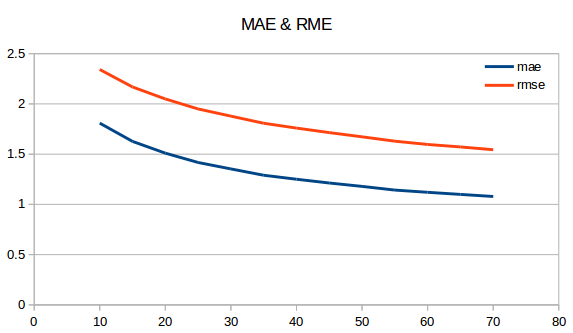
\includegraphics[width=200pt, height=140pt]{img/mae_rmse.png}
		\caption{Métricas MAE \& RMSE.}
		\label{mae_rmse}
	\end{figure}
	
	Como se puede comprobar, el comportamiento de ambas es el mismo (de hecho su computación solo varía en el valor de una constante) y en general mejoran según aumenta el número de vecinos que usamos para realizar la recomendación.
	
	\section{Análisis de redes sociales}
	
	En la figura \ref{distribuciones} podemos ver las distribuciones de grado que siguen las diferentes redes sociales.
	
	\begin{figure}[ht!]
		\begin{subfigure}[t!]{\textwidth}
			\begin{subfigure}[t!]{\textwidth}
				\centering
				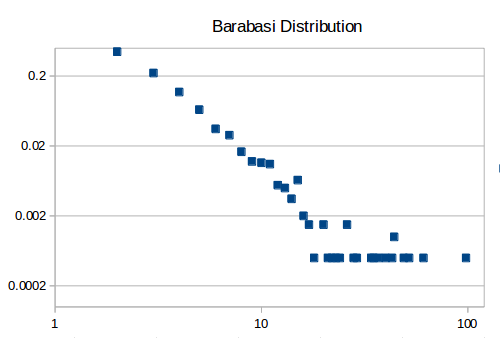
\includegraphics[width=180pt, height=120pt]{img/barabasi_dl.png}
			\end{subfigure}\\
			\begin{subfigure}[t!]{\textwidth}
				\centering
				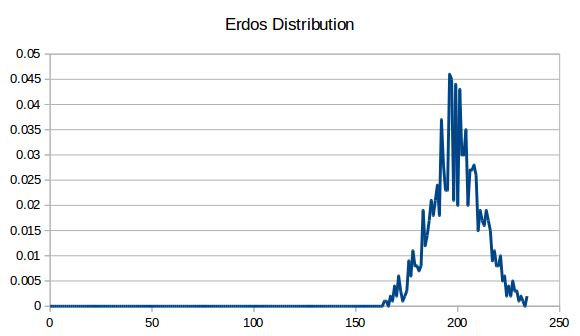
\includegraphics[width=180pt, height=120pt]{img/erdos_d.png}
			\end{subfigure}
		\end{subfigure}
		\begin{subfigure}[t!]{\textwidth}
			\begin{subfigure}[t!]{\textwidth}
				\centering
				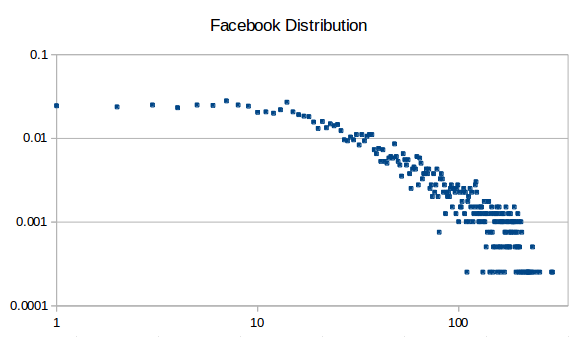
\includegraphics[width=180pt, height=120pt]{img/facebook_dl.png}
			\end{subfigure}
			\begin{subfigure}[t!]{\textwidth}
				\centering
				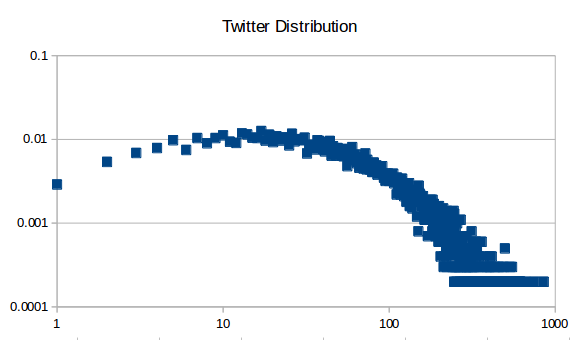
\includegraphics[width=180pt, height=120pt]{img/twitter_d.png}
			\end{subfigure}
		\end{subfigure}
		\caption{%
			Distribuciones de grado.
		}%
		\label{distribuciones}
	\end{figure}
	
	Como se puede comprobar, el grafo Barabasi sigue una distribución powerlaw y el grafo Erdos una normal de media 200 
	(se han usado 1000 nodos y una probabilidad de enlace de 0.2). La distribución de Facebook también se corresponde con 
	los modelos vistos en teoría y es bastante similar a la de twitter, para la que se ha considerado un grafo no dirigido.\\
	
	En las gráficas de la figura \ref{scatters} podemos ver los scatterplots de pagerank y betweenness.\\
	
		\begin{figure}[ht!]
			\begin{subfigure}[t!]{0.5\textwidth}
				\begin{subfigure}[t!]{\textwidth}
					\centering
					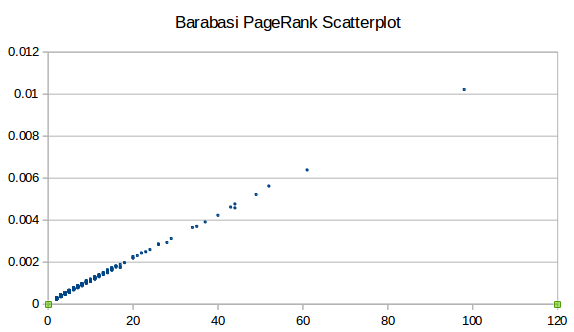
\includegraphics[width=180pt, height=120pt]{img/barabasi_pr_s.png}
				\end{subfigure}\\
				\begin{subfigure}[t!]{\textwidth}
					\centering
					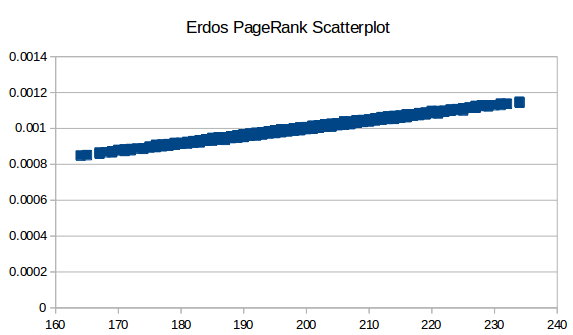
\includegraphics[width=180pt, height=120pt]{img/erdos_pr_s.png}
				\end{subfigure}
			\end{subfigure}
			\begin{subfigure}[t!]{0.5\textwidth}
				\begin{subfigure}[t!]{\textwidth}
					\centering
					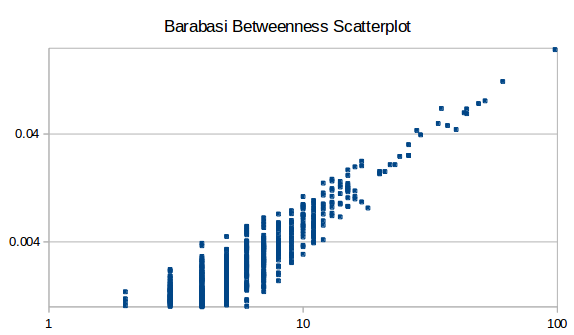
\includegraphics[width=180pt, height=120pt]{img/barabasi_b_s.png}
				\end{subfigure}
				\begin{subfigure}[t!]{\textwidth}
					\centering
					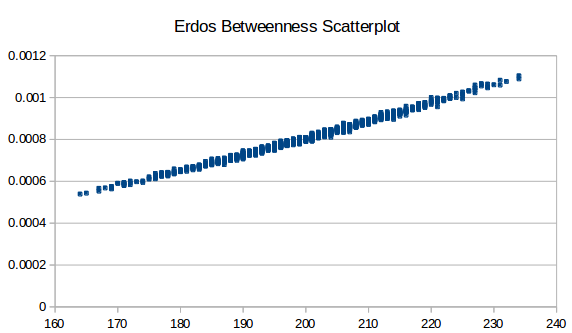
\includegraphics[width=180pt, height=120pt]{img/erdos_b_s.png}
				\end{subfigure}
			\end{subfigure}
			\begin{subfigure}[t!]{0.5\textwidth}
				\begin{subfigure}[t!]{\textwidth}
					\centering
					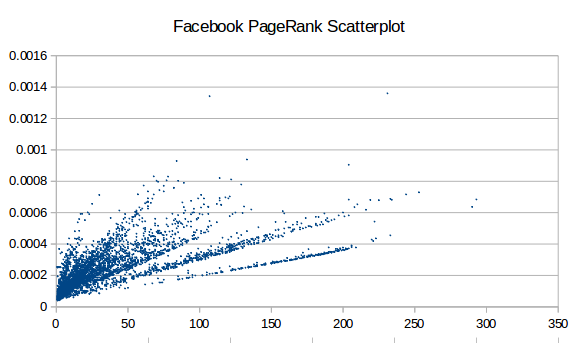
\includegraphics[width=180pt, height=120pt]{img/facebook_pr_s.png}
				\end{subfigure}
				\begin{subfigure}[t!]{\textwidth}
					\centering
					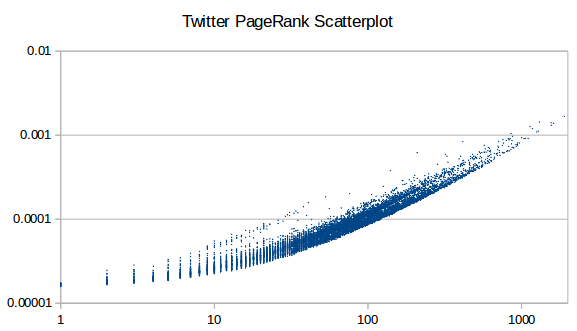
\includegraphics[width=180pt, height=120pt]{img/twitter_pr_s.png}
				\end{subfigure}
			\end{subfigure}
			\begin{subfigure}[t!]{0.5\textwidth}
				\begin{subfigure}[t!]{\textwidth}
					\centering
					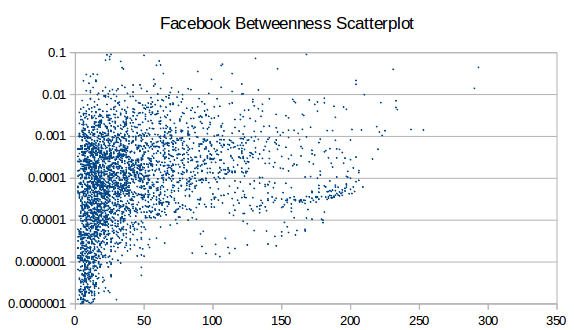
\includegraphics[width=180pt, height=120pt]{img/facebook_b_s.png}
				\end{subfigure}
				\begin{subfigure}[t!]{\textwidth}
					\centering
					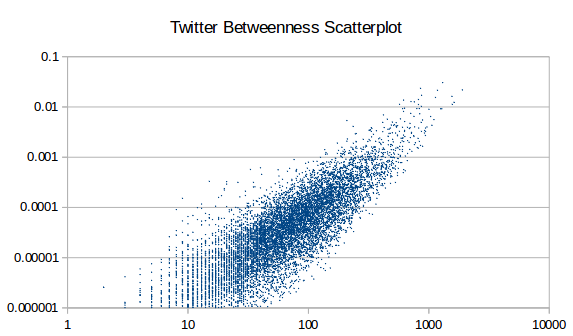
\includegraphics[width=180pt, height=120pt]{img/twitter_b_s.png}
				\end{subfigure}
			\end{subfigure}
			\caption{%
				Scatterplots
			}%
			\label{scatters}
		\end{figure}
	
	En la siguiente tabla podemos ver el número de puentes locales encontrados en las redes, así como el ratio respecto a número total de enlaces:

	\begin{center}
		\begin{tabular}{|c|c|c|c|}
			\hline
			&\textbf{Puentes Locales} & \textbf{Puentes totales} & \textbf{Ratio} \\ 
			\hline
			Barabasi & 3882 & 3994 & 97.19\% \\
			\hline
			Erdos & 0 & 99696 & 0\% \\
			\hline
			Facebook & 704 & 84232 & 0.8\% \\
			\hline
			Twitter & 6884 & 560227 & 1.2\% \\
			\hline
		\end{tabular}
	\end{center}	
	
	El grafo Barabasi ha sido generado con 2 enlaces por nodo, por lo tanto es muy poco probable que dos nodos tengan un amigo en común, por eso es tan alto
	el número de puentes locales.
	Esto no es así en facebook ni twitter, y menos aún en el grafo Erdos, en el que cada nodo tiene una media de 200 conexiones, de forma que es altamente probable
	(en esta ejecución en concreto, tiene probabilidad 1) que alguno de nuestros 200 contactos (que a su vez tienen una media de 200 contactos) esté conectado con alguno de los 800 individuos con los que no estamos conectados directamente.\\
	
	A continuación se muestra una tabla con el porcentaje de nodos en cada red social que cumplen la paradoja de la amistad.
	\begin{center}
		\begin{tabular}{|c|c|c|c|c|}
			\hline
			\textbf{Barabasi} & \textbf{Erdos} & \textbf{facebook4k} & \textbf{twitter10k} \\ 
			\hline
			86.8 \% & 53.4\% & 76\% & 89.62\% \\
			\hline
		\end{tabular}
	\end{center}
	En diversas ejecuciones de Erdos, se ha encontrado un porcentaje por debajo del 50\%, por lo que podemos concluir que generalmente no se cumple la paradoja.
	En el resto de redes sí se cumple la paradoja.
	
\end{document}